\chapter{Feedback Linearization}

\section{Introduction}

Feedback linearization has been successfully applied to a wide range of nonlinear systems, including robotic manipulators, aerospace vehicles, and chemical processes. It provides a systematic approach to control design and can significantly improve the performance and stability of nonlinear systems.

In the following sections, we will explore the mathematical foundations of feedback linearization, discuss its application to various systems, and present examples to illustrate its effectiveness. We will also look at an interesting class of systems called \textbf{Mechanically Feedback Linearizable} systems, which can be controlled using feedback linearization techniques.

\section{Feedback Linearization}

Feedback linearization is a control technique used to transform a nonlinear system into an equivalent linear system through a change of variables and a suitable feedback control law. This method allows the application of linear control techniques to nonlinear systems, which can simplify the design and analysis of control systems.

Consider the following continuous-time dynamical system (for $t \in [0, T ], T > 0$):

\begin{equation}
    \label{eq:cts}
    \dfrac{d}{dt}x(t) = X(x(t), u(t))
\end{equation}

on an $n$-dimensional manifold $M$, where $X(\cdot, u) \in \mathfrak{X}(M)$ is a vector field, for each $u \in U \subset \R[n]$. A point $(x_0, u_0) \in M \times U$ is called an equilibrium point of the system~\eqref{eq:cts} if $X(x_0, u_0) = 0$.

\begin{defn}
    Let $M$ and $N$ be two $n$-dimensional manifolds and $\varphi: M \lra N$ be a diffeomorphism. Let $X \in \mathfrak{X}(M)$ be a vector field on $M$. Then, $X_{\varphi} = T\varphi \circ X \circ \varphi^{-1}$ is a vector field on $N$ (push-forward) for the dynamical system
    \begin{equation}
        \dfrac{d}{dt}\tilde{x}(t) = X_{\varphi}(\tilde{x}(t), u(t))
    \end{equation}
    with $\tilde{x}(0) = \varphi(x(0))$ satisfying $\tilde{x}(t) = \varphi(x(t)), t \in [0,T]$.

    Let $x \in \mathcal{O}(x_0)$ and $u \in \mathcal{O}(u_0)$ be open balls (neighborhood) around $x_0$ and $u_0$ in $M$ and $U$ respectively. Let $x \mapsto \varphi(x) = \tilde{x} \in N : = \R[n]$ be a diffeomorphism, and $(x,u) \mapsto \psi(x,u) : = v \in \R[m]$ such that for each fixed $x$, $\psi(x, \cdot) : U \lra \R[n]$ is invertible. Thus, a dynamical system \eqref{eq:cts} is said to be (locally) feedback linearizable around $(x_0, u_0)$ on $\mathcal{O}(x_0) \times \mathcal{O}(u_0)$ if there exists matrices $A \in \R[n \times n]$ and $B \in \R[n \times m]$ such that $X_{\varphi}(\tilde{x}, v) = A \tilde{x} + Bv$, with $v = \psi(\varphi^{-1}(\tilde{x}), u)$. The feedback linearized dynamical system is given by:

    \begin{equation}
        \dfrac{d}{dt}\tilde{x}(t) = A \tilde{x}(t) + B v(t)
    \end{equation}
\end{defn}

\subsection{Example}

Consider the following continuous-time dynamical system:
    \begin{equation}
        \pmat{\dot{x}_1 \\ \dot{x}_2} = \pmat{(1+2u(t))x_2(t) \\ u(t)}
    \end{equation}

Taking $\tilde{x}_1 = x_1 - x_2^2$ and $\tilde{x}_2 = x_2$, we get the diffeomorphism $\varphi(x_1, x_2) = \left(x_1 - x_2^2, x_2 \right)$, we get the feedback linearized system:

\begin{equation}
    \pmat{\dot{z}_1(t) \\ \dot{z}_2(t)} = \pmat{z_2(t) \\ u(t)}
\end{equation}

\subsection{Discrete Feedback Linearization}

Let's take a detour and check if a discretized system is feedback linearizable. Consider the same example as above.

First, we consider the forward Euler discretization scheme $\D(x, v) = (x, x + v)$. This gives a discrete-time system:

\begin{equation}
    \pmat{x_{1,k+1} \\ x_{2, k+1}} = \pmat{x_{1,k} \\ x_{2,k}} + h\pmat{(1+2u_k)x_{2,k} \\ u_k}
\end{equation}

Taking the same diffeomorphism $\varphi$ as before, we get:

\begin{equation}
    \pmat{z_{1,k+1} \\ z_{2,k+1}} = \pmat{z_{1,k} + hz_{2,k} - h^2 u_k^2 \\ z_{2,k} + h u_k}
\end{equation}

Thus, we see that it is NOT feedback linearizable.

Now, let's consider an alternate discretization which yields the discrete system:

\begin{equation}
    \pmat{x_{1,k+1} \\ x_{2, k+1}} = \pmat{x_{1,k} \\ x_{2,k}} + h\pmat{(1+2u_k)x_{2,k} \\ u_k} + h^2 \pmat{u_k^2 \\ 0}
\end{equation}

Again taking the same diffeomorphism $\varphi$, we get:

\begin{equation}
    \pmat{z_{1,k+1} \\ z_{2,k+1}} = \pmat{z_{1,k} + hz_{2,k} \\ z_{2,k} + h u_k}
\end{equation}

which is indeed feedback linearizable.

Thus, we see that the choice of discretization scheme can affect the feedback linearizability of a system.


\section{Feedback Linearizable Discretization}


\begin{figure}[h]
    \centering
    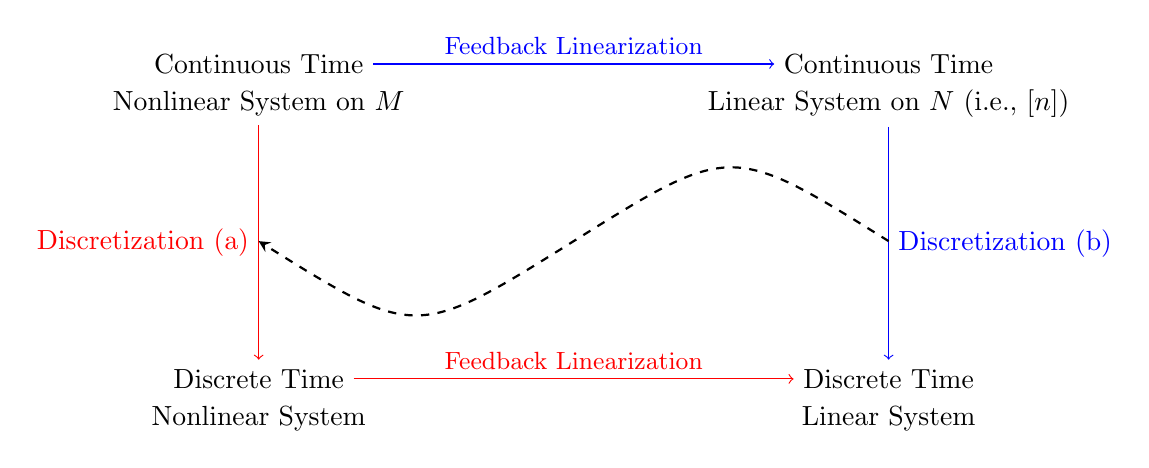
\begin{tikzpicture}
        \node (CTNS) at (0,0) {Continuous Time};
        \node (CTNS-2) at (0, -0.5) {Nonlinear System on $M$};
        \node (CTLS) at (8,0) {Continuous Time};
        \node (CTLS-2) at (8,-0.5)  {Linear System on $N$ (i.e., $\R[n]$)};
        \node (DTNS) at (0,-4) {Discrete Time};
        \node (DTNS-2) at (0, -4.5) {Nonlinear System};
        \node (DTLS) at (8,-4) {Discrete Time};
        \node (DTLS-2) at (8, -4.5)  {Linear System};
        \draw[->, blue] (CTNS) -- node[above]{\small{Feedback Linearization}} (CTLS);
        \draw[->, red] (DTNS) -- node[above]{\small{Feedback Linearization}} (DTLS);
        \draw[->, red] (CTNS-2) -- node[left]{Discretization (a)} (DTNS);
        \draw[->, blue] (CTLS-2) -- node[right]{Discretization (b)} (DTLS);

        \draw[dashed, thick, ->, >=stealth] (8, -2.25) .. controls (6,-1) .. (4, -2.25) .. controls (2,-3.5) ..  (0, -2.25);
    \end{tikzpicture}
    \caption{Feedback Linearizable Discretization}
\end{figure}

As seen from above, the following question persists: \textsl{Given a feedback linearizable continuous-time system, is it possible to construct a numerical discretization which is also feedback linearizable?}

Yes. We can do this by using the notion of lifts of discretization maps, since the feedback linearization is a diffeomorphism. Invoking the proposition~\eqref{prop:retr-lift}, we can construct a discretization scheme:

\begin{equation}
    \left(\D^{TM}\right)^{-1}(x_k, x_{k+1}) = hX \left( \tau_M \left( \left( \D^{TM} \right)^{-1} \left( x_k, x_{k+1}\right), u_k  \right) \right) 
\end{equation}

\begin{equation}
    \D^{TN} = (T\varphi \times T \varphi)^{-1} \circ \D^{TM} \circ TT \varphi
\end{equation}

This allows us to define a scheme on $TM$ for a choice of discretization on $TN$, and a given change of coordinates $\varphi$ via feedback linearization.


\section{Mechanical Feedback Linearization}
Mechanical Feedback Linearization (MF-Linearization) is the application of feedback linearization to nonlinear mechanical systems. Mechanical systems usually evolve on a configuration manifold $M$, hence feedback linearization would usually not yield a linear system which preserves the mechanical structure (due to the affine connection). 

However, there exists a class of mechanical systems, called the \textbf{MF-Linearizable} systems, for which feedback linearization is possible:

\begin{defn}
    A mechanical control system $(\mathcal{MS})_{(n,m)} = (M, \nabla, \mathfrak{g}, e)$ is called $MF$-linearizable if it is $MF$-equivalent to a linear mechanical system $(\mathcal{LMS})_{(n,m)} = (\R[n], \overline{\nabla}, \mathfrak{b}, A \widetilde{x})$, where $\overline{\nabla}$ is an affine connection with the Christoffel symbols zero ($\overline{\nabla}$ is a flat connection) and $\mathfrak{b} = \{b_1, \dots, b_m \}$ are constant vector fields. In other words, there exists $(\varphi, \alpha, \beta, \gamma) \in MF$ such that 
    \begin{equation}
        \begin{split}
            \varphi: M \lra N \ \ \varphi(x)  &= \widetilde{x} \\
            \varphi_*\left(\nabla - \sum_{r=1}^m g_r \otimes \gamma^r\right) &= \overline{\nabla} \\
            \varphi_*\left( \sum_{r=1}^m \beta^r_s g_r \right) &= b_s, \ 1 \leq s \leq m \\
            \varphi_* \left( e + \sum_{r=1}^m g_r \alpha^r \right) &= A \widetilde{x}
        \end{split}
    \end{equation}
    Equivalently, we have the corresponding linear mechanical system $(\mathcal{LMS})_{(n,m)}$ as:
    \begin{equation}\label{sode-lin}
            \dot{\tilde{x}}  = \tilde{y}; \ 
            \dot{\tilde{y}}  = A \tilde{x} + \sum_{s=1}^m b_s \tilde{u}_s
    \end{equation}
\end{defn}


\subsection{Determining MF-Linearizability}

\textsl{Given a mechanical system, how do we determine if it falls under the class of mechanically feedback linearizable systems?}

From the definition in~\eqref{eq:mech}, we can define the following distributions:

\begin{equation}
    \begin{split}
        \mathcal{E}^0 & = \text{span} \{ g_r, 1 \leq r \leq m \} \\
        \mathcal{E}^j & = \text{span} \{ \text{ad}^i_e g_r, 1 \leq r \leq m, 0 \leq i \leq j \}
    \end{split}
\end{equation}

Thus, we state the following theorem:
\begin{thm}\label{thm:mfl}
    A mechanical system $(\mathcal{MS})_{(n,m)}$ is said to be mechanical feedback ($MF$) linearizable, locally around $x_0 \in M$ if and only if, in the neighborhood of $x_0$, it satisfies the following conditions:

    \begin{itemize}
        \item $(ML1)$ $\mathcal{E}^0$ and $\mathcal{E}^1$ are of constant rank
        \item $(ML2)$ $\mathcal{E}^0$ is involutive
        \item $(ML3)$ $\text{ann } \mathcal{E}^{0} \subset \text{ann } \mathfrak{R}$
        \item $(ML4)$ $\text{ann } \mathcal{E}^0 \subset \text{ann } \nabla g_r \ \forall r: 1 \leq r \leq m$
        \item $(ML5)$ $\text{ann } \mathcal{E}^1 \subset \text{ann } \nabla^2 e$
    \end{itemize}
where $\mathfrak{R}$ is the Riemannian curvature tensor and $\text{ann}$ is the annihilator.
\end{thm}

\begin{rmk}
    The above conditions $(ML1)$--$(ML5)$ are valid without the assumption of controllability of the linearized mechanical system
\end{rmk}

We can also define the feedback linearization for different classes of mechanical systems. The following proposition is explicitly stated for planar mechanical systems where $n=2$. (refer~\cite{nowicki}).

\begin{prop}
\label{prop:planar_mech}
A planar mechanical system $\mathcal{(MS)}_{(2,1)}$ is locally $MF$-linearizable at $x_0 \in M$ to a controllable $\mathcal{(LMS)}_{(2,1)}$, if and only if it satisfies the following conditions:
\begin{enumerate}
    \item $(MD1)$ $g$ and $\text{ ad}_e g$ are independent
    \item $(MD2)$ $\nabla_g g \in \mathcal{E}^0$ and $\nabla_{\text{ad}_e g} g \in \mathcal{E}^0$
    \item $(MD3)$ $\nabla^2_{g, \text{ad}_e g} \text{ad}_e g - \nabla^2_{\text{ad}_e g, g} \text{ad}_e g \in \mathcal{E}^0$
\end{enumerate}
\end{prop}